\section{Simple Operations on Signals}
%-----------------Transformations of the Time Variable--------------------%
 \subsection{Transformations of the Time Variable}
 \begin{itemize}
 \item Time delay
 \item Time reversal 
 \item Time scaling
 \end{itemize}
\begin{figure}[H]
    \centering 
    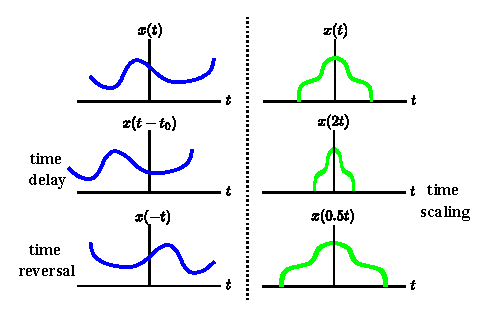
\includegraphics[width=.7\textwidth]{images/transformation.eps}
    \caption{Transformations applies to the time variable: time delay (left middle), time reversal (left bottom), time scaling (right)} 
\end{figure}
%-----------------Amplitude Transformation--------------------%
  \subsection{Amplitude Transformation}
  \[ y(t) = Ax(t)+B \]
  \quad where $A,B$ are constants.
%-----------------Linear Combination--------------------%
\subsection{Linear Combination}
\begin{itemize}
\item In continuous-time domain:
\[ y(t) = a_{1}x_{1}(t)+a_{2}x_{2}(t)+...+a_{N}x_{N}(t) \]
\item In discrete-time domain:
\[ y[n] = a_{1}x_{1}[n]+a_{2}x_{2}[n]+...+a_{N}x_{N}[n] \]
 \quad where $a_{i} \in \mathbb{C}$, $i=1,2,...,N$ are real or complex numbers.
\end{itemize}
%-----------------Multiplication--------------------%
\subsection{Multiplication} 
\begin{itemize}
\item In continuous-time domain: 
\[ y(t) = x_{1}(t) \cdot x_{2}(t) \]
\item In discrete-time domain:
\[ y[n] = x_{1}[n] \cdot x_{2}[n] \]
\end{itemize}
This implies \textbf{instantaneous multiplication} for each time instant or each discrete time sample.
%-----------------Scaler product and norm--------------------%
\subsection{Scalar Products and Norms}
%-----------------Scaler product and norm of vectors--------------------%
\subsubsection{Scalar Product and Norm of Vectors}
\begin{itemize}
\item The \textbf{scalar product} between two 3-D vectors $\vec{A}$ and $\vec{B}$: projection of $\vec{A}$ on $\vec{B}$.
\[ \vec{A} \cdot \vec{B} = A_{x} \cdot B_{x} + A_{y} \cdot B_{y} + A_{z} \cdot B_{z} = \lvert \vec{A} \rvert \cdot \lvert \vec{B} \lvert \cos(\phi) \]
%The \textbf{scaler} product between the 3D vectors $\vec{A}$ and $\vec{B}$ is computed as the sum of the multiplication between entries $(A_{x} \cdot B_{x} + A_{y} \cdot B_{y} + A_{z} \cdot B_{z})$, or equivalently as $A\cdot B \cos(\phi)$, where $A$ and $B$ is the lengths of the vectors and $\phi$ is the angle between them.
 \item For vectors, the \textbf{Euclidean norm}, or \textbf{norm-2}, is the length of vectors in Euclidean space:
 \[ \lvert \lvert \vec{A} \rvert \rvert_{2} = \sqrt{\vec{A} \cdot \vec{A}} = A = \sqrt{A_{x}^2+A_{y}^2+A_{z}^2} \]
 \end{itemize}
 %-----------------Scalar Product and Norm of Discrete-time Signals--------------------%
 \subsubsection{Scalar Product and Norm of Discrete-time Signals}
 \begin{itemize}
    \item \textbf{Scalar product} (or, inner product) between two discrete-time signals, $x_1[n]$ and $x_2[n]$:
    \[
        \langle x_{1}[n], x_{2}[n] \rangle = \sum_{n=-\infty}^{\infty} x_{1}[n] x_{2}^{*}[n]
    \]
    
    \item \textbf{Norm-2} for a discrete-time signal $x[n]$:
    \[
        \lvert \lvert x[n] \rvert \rvert_{2} 
        = \sqrt{\langle x[n], x[n] \rangle}
        = \sqrt{\sum_{n=-\infty}^{\infty} \lvert x[n] \rvert^{2}} 
        = \left( \sum_{n=-\infty}^{\infty} \lvert x[n] \rvert^{2} \right) ^{\frac{1}{2}}
    \]
    norm-2 is the square root of the \textbf{energy} of the signal
    
    \item \textbf{Norm-$p$} for a discrete-time signal, $x[n]$:
    \[
        \lvert \lvert x[n] \rvert \rvert_{p} \ 
        = \ \left( \sum_{n=-\infty}^{\infty} \lvert x[n] \rvert^{p} \right)^{\frac{1}{p}}, 
        \quad \text{for} \ 1 \leq p < \infty
    \]
    \begin{itemize}
        \item For $p=1$ (norm-1):
        \[
            \lvert \lvert x[n] \rvert \rvert_{1} \ 
            = \ \sum_{n=-\infty}^{\infty} \lvert x[n] \rvert 
        \]
        
        \item For $p \to \infty$: infinity norm / maximum norm:
        \[
            \lvert \lvert x[n] \rvert \rvert_{\infty} \ = \ \max_{n} \lvert x[n] \rvert 
        \] 
    \end{itemize}
    
    \item Norms are measures of the signal “strength”. Each norm is a different way of measuring signal strength. \textit{E.g.,} norm-2 is associated with the energy.
    
    \item The space of signals with a finite norm-$p$ is called $L^{p}$ space.
\end{itemize}
 
 %-----------------Scalar Product and Norm of Continuous-time Signals--------------------%
\subsubsection{Scalar Product and Norm for Continuous-time Signals}
\begin{itemize}
    \item \textbf{Scalar product} (or, inner product) between two continuous-time signals, $x_1(t)$ and $x_2(t)$:
    \[
        \langle x_{1}(t), x_{2}(t) \rangle \ = \ \int_{-\infty}^{+\infty}  x_{1}(t) x_{2}^{*}(t) \mathrm{d}t 
    \]
    where $x_{2}^{*}(t)$ denotes the complex conjugate of $x_2(t)$ - this can be ignored if the signal only has the real part.
    
    \item \textbf{Norm-2} for the continuous-time signal,  $x(t)$:
    \[ 
        \lvert \lvert x(t) \rvert \rvert_{2} = \sqrt{\langle x(t), x(t) \rangle} = \sqrt{\int_{-\infty}^{+\infty}\lvert x(t) \rvert^{2} \mathrm{d}t} = \left( \int_{-\infty}^{\infty} \lvert x(t) \rvert^{2} \right) ^{\frac{1}{2}} 
    \]
    
    \item \textbf{Norm-$p$} for the continuous-time signal, $x(t)$:
    \[
        \lvert \lvert x(t) \rvert \rvert_{p} =\left( \int_{-\infty}^{+\infty} \lvert x(t) \rvert^{p} \mathrm{d}t \right)^{\frac{1}{p}}\quad ; \quad \lvert \lvert x(t) \rvert \rvert_{\infty} \ = \ \max_{n}  \lvert x(t) \rvert 
    \]
\end{itemize}

%==============================================%
% inner product example
\begin{q}{}
The signal $f_1(t)$ is defined as
\[
    f_1(t) = \begin{cases}
        \lvert t \rvert, & \lvert t \rvert \leq \pi \\
        0, & \text{otherwise}
    \end{cases}
\]
and the signal $f_2 (t)$ is defined as
\[
    f_2 (t) = -2 \sin(2t)
\]
The inner product between the signals $f_1(t)$ and $f_2(t)$ is:
\begin{multicols}{2}
\begin{enumerate}[label=(\alph*)]
    \item 3
    \item 1
    \item $\pi$
    \item 0
\end{enumerate} 
\end{multicols}
\end{q}
 
%-----------------Characterising similarity/difference between signals--------------------%
\subsection{Characterising Similarity/Difference Between Signals}
\subsubsection{Measuring the Similarity}
Normalizing the scalar product between two \textit{2-dimensional} vectors ($\vec{A} \cdot \vec{B}$) to the lengths of the vectors ($\lvert \vec{A} \rvert$ and $\lvert \vec{B} \rvert$) gives out the information of direction between two vectors,
\[
    \vec{A} \cdot \vec{B} =\lvert \vec{A} \rvert \cdot \lvert \vec{B} \rvert \cos(\phi)
    \quad \Rightarrow \quad 
    \cos(\phi) = \frac{\vec{A} \cdot \vec{B}}{\lvert \vec{A} \rvert \cdot \lvert \vec{B} \rvert}
    \in [-1, 1]
\]
\begin{itemize}
    \item if $\cos(\phi) = 1$, $\vec{A}$ and $\vec{B}$ are parallel;
    \item if $\cos(\phi) = -1$, $\vec{A}$ and $\vec{B}$ are anti-parallel;
    \item if $\cos(\phi) = 0$, $\vec{A}$ and $\vec{B}$ are orthogonal.
\end{itemize}
A similar idea applies to measuring how similar two signals are - we \textit{normalise} the scalar (inner) product between two signals by norm-2 of the signals. This is called the \textbf{normalised scalar product} between two signals\footnote{signals are commonly in high dimensions, the angle between two signals are not easy to visualise, but the computation carries the same idea as how we treat 2D vectors!}.

\begin{itemize}
    \item For two \textit{continuous-time} signals,
    \[
        \cos(\phi) = \frac{\langle x_{1}(t), x_{2}(t) \rangle}{ \lvert \lvert x_{1}(t) \rvert \rvert_{2} \ \lvert \lvert x_{2}(t) \rvert \rvert_{2}};
    \]
    
    \item for two \textit{discrete-time} signals,
    \[
        \cos(\phi) = \frac{\langle x_{1}[n], x_{2}[n] \rangle}{ \lvert \lvert x_{1}[n] \rvert \rvert_{2} \ \lvert \lvert x_{2}[n] \rvert \rvert_{2}}.
    \]
\end{itemize}


\subsubsection{Cross-correlation Function and Normalized Cross-correlation Function}
\begin{itemize}
    \item In practical conditions, signals are commonly corrupted by noise. 
    \begin{figure}[H]
        \centering 
        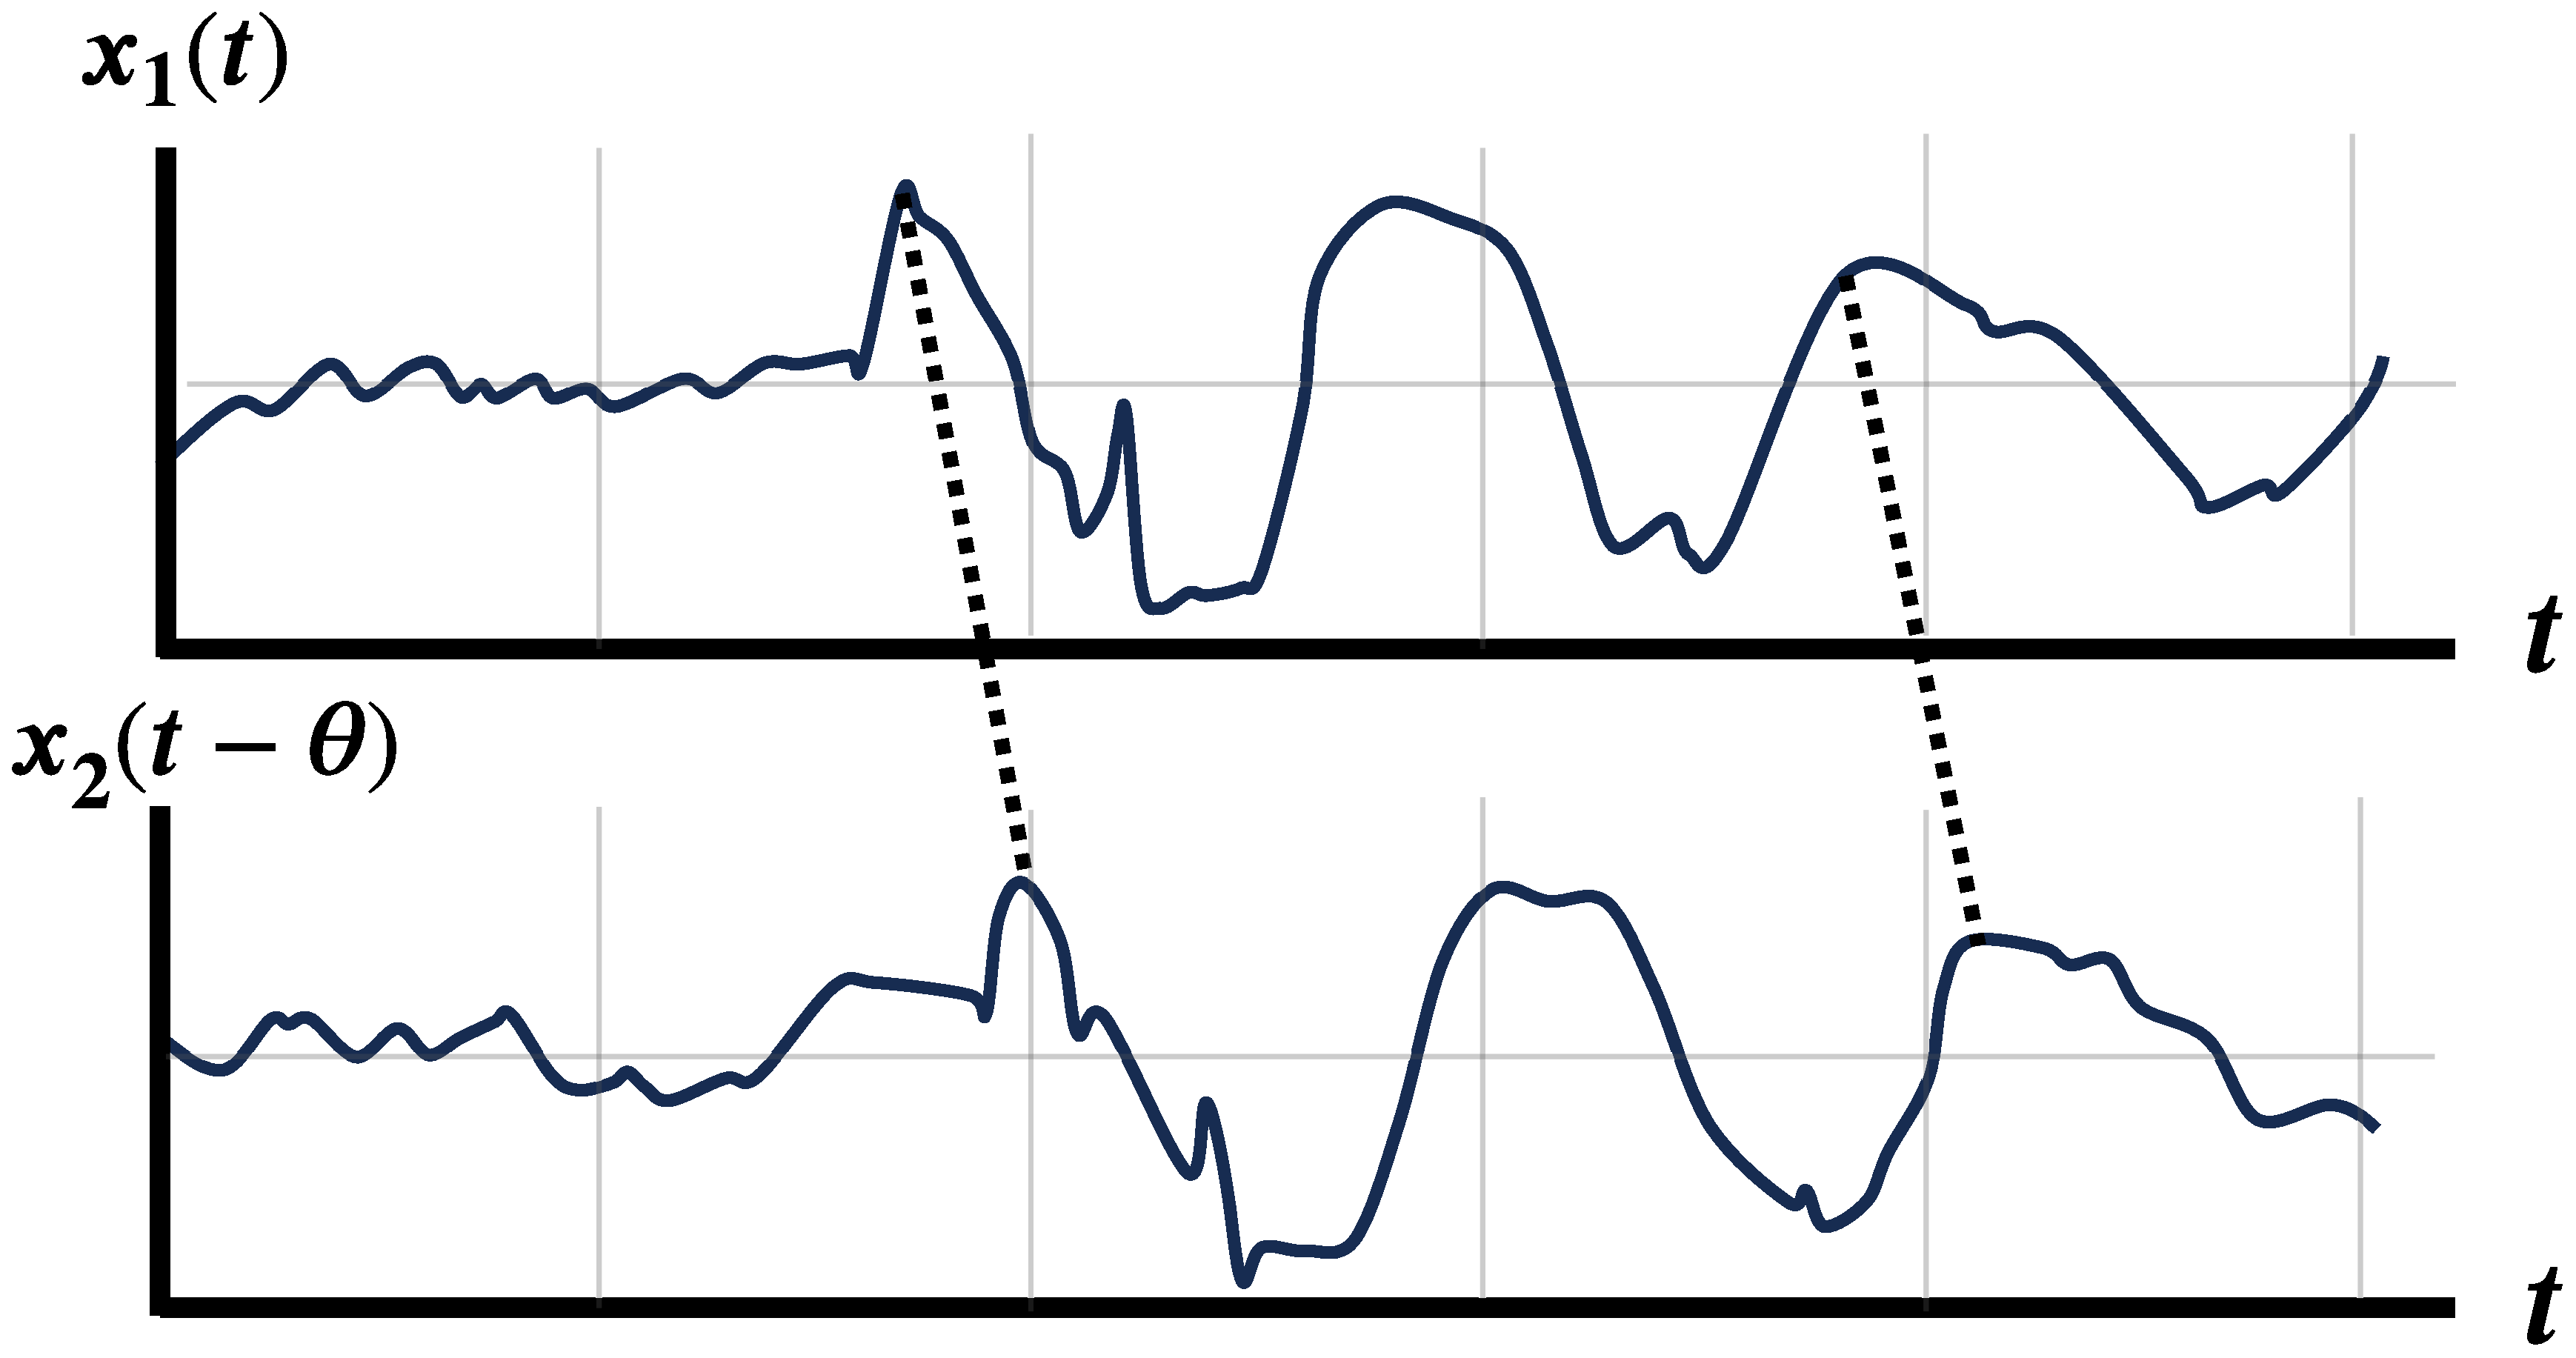
\includegraphics[width=0.6\textwidth]{images/correlation.eps}
        \caption{Two signals corrupted by noise, but they are correlated by shifting $x_2(t)$ with the time delay $\theta$} 
    \end{figure}
    
    \item A possible estimate of the delay between the two signals is the time interval by which we need \textbf{to shift one of the signals so that it is maximally similar to the other}, \textit{i.e.}, determining the shift, $\theta$, at which two signals are in best temporal alignment.
\end{itemize}

\paragraph{Cross-correlation function, $c(\theta)$} The cross-correlation function is defined as the scalar product between the signal $x_1(t)$ and the \textit{shifted} signal $x_2(t-\theta)$,
\[
    c(\theta) = \langle x_1(t), x_2(t-\theta) \rangle,
\]
where our objective is finding the best value of $\theta$ that could maximise the cross-correlation function, \textit{i.e.}, find the max similarity between two signals,
\[
    \theta_{\text{best}} = \argmax_{\theta \in \mathbb{R}} c(\theta).
\]
\textit{A special case} of the cross-correlation is \textbf{auto-correlation}, where similarity is measured between $x(t)$ and $x(t-\theta)$, \textit{i.e.}, to the signal itself,
\[
    a(\theta) = \langle x(t), x(t-\theta) \rangle,
\]
which can be useful to say how quickly a signal is changing characteristics in some way (\textit{e.g.}, ultrasonic signal).

\paragraph{Normalized cross-correlation function, $f_c(\theta)$} The normalised cross-correlation function is defined as the normalised scalar product of the cross-correlation function, 
\begin{align*}
\begin{split}
    f_{c}(\theta)
    &= \frac{\langle x_{1}(t), x_{2}(t-\theta) \rangle}{ \lvert \lvert x_{1}(t) \rvert \rvert_{2} \ \lvert \lvert x_{2}(t) \rvert \rvert_{2}} \\\\
    &= \frac{\int_{-\infty}^{\infty}  x_{1}(t) x_{2}(t-\theta) \mathrm{d}t}{\sqrt{\int_{-\infty}^{+\infty}\lvert x_{1}(t)
    \rvert^{2} \mathrm{d}t} \cdot \sqrt{\int_{-\infty}^{+\infty}\lvert x_{2}(t-\theta) \rvert^{2} \mathrm{d}t}}.
\end{split}
\end{align*}

\begin{ex}{- Measure muscle fiber conduction velocity}
    \begin{minipage}{0.4\textwidth}
    \includegraphics[width=\textwidth]{images/emg3}
    \end{minipage}\hfill
    \begin{minipage}{0.4\textwidth}
    \includegraphics[width=\textwidth]{images/emg1}
    \end{minipage}
    \ \\
    By applying the cross-correlation function, we are able to find the time delay between two EMG signals. By measuring the distance between two electrodes, we can calculate the conduction velocity.
    \begin{figure}[H] 
        \centering
        \includegraphics[width=0.5\textwidth]{images/emg2}
    \end{figure}
\end{ex}
 
 
\subsubsection{Measuring the Difference}
\begin{itemize}
    \item An alternative way to measure the similarity between two signals is computing the \textbf{strength of their difference} (\textit{i.e.}, norm). 

    \item For example, using norm-2 to measure the strength of difference, we define the \textbf{mean squared error (MSE)} between two signals:
    \begin{align*} 
    \begin{split} 
        MSE(\theta) 
        &= \lvert \lvert x_{1}(t) - x_{2}(t-\theta) \rvert \rvert_{2}^{2}\\
        &=\int_{-\infty}^{+\infty} \lvert x_{1}(t) - x_{2}(t-\theta) \rvert^{2} \mathrm{d}t
    \end{split} 
    \end{align*}
    where
    \begin{itemize}
        \item $MSE(\theta)$ is a function of the shift $\theta$;
        \item the minimum value of $\theta$ best estimates the delay;
        \item MSE is the energy of the error signal.
    \end{itemize}
\end{itemize}